\chapter{Considering the case of \texorpdfstring{$N=2$}{N=2}}
\label{ch:2p}

When moving to higher dimensions, 
    it gets difficult to visualize the solutions.
The $N=2$ case can still be visualized without getting too abstract.

For this special case, we choose a symmetric arrangement around the global origin where $d_1 = -d_2$.
As such, we can describe the particle positions by $l := |d_1 - d_2| = 2|d_1|$.
With that, we may reformulate our condition as 
\begin{equation}
    k_c \frac l2 = n \pi.
\end{equation}
This condition can be reformulated as
\begin{equation}
    l = n \lambda_c.
\end{equation}
To satisfy the assumption that the tweezers don't affect each other,
    we choose $n=2$.

From the definition of the detuning \eqref{eq:sp:def:detuning},
    we can generate this expression
\begin{equation}
        \lambda_c 
            = \lambda_0 \frac{1}{\frac\Delta{\omega_0} +1} 
            \approx \lambda_0 \left(1 - \frac{\Delta}{\omega_0}\right)
\end{equation}
which gives $\lambda_c$ dependent on the detuning
    and thus $l$ in dependence of the detuning.
Since we only have two particles, we will define $\phi_1 = 0$ and $\phi_2 = \phi$.

The results of the calculation can be seen in Figure \ref{fig:2p:phi0} and Figure \ref{fig:2p:phi10}.
Figure \ref{fig:2p:phi0} shows the system with a phase of $\phi = 0$ 
    and Figure \ref{fig:2p:phi10} shows the system with a phase of $\phi = \pi/10$.
From Figure \ref{fig:2p:phi0} we may see how the solutions lie in the quadrants I, II, and IV. \footnote{
Quadrant I...$z_1, z_2 > 0$ and II and IV...$z_1 = -z_2$
}
It can be observed that the solutions contract around the origin with rising detuning values.
The solutions also lie along a loop in the II and IV quadrants,
    which become wider and move towards the origin with increasing detuning values.

It is also interesting to observe the asymmetry when adding a phase difference between the tweezers.
%We can interpret the introduction of the phase shift as a non-linear rescaling of $z_2$.
As expected, the symmetry when exchanging $z_1$ and $z_2$ is broken when $\phi_1 \neq \phi_2$.

The solutions lie on a $1$-dimensional manifold, when considering $z_1$ vs $z_2$.
Since we can assume that the solutions vary smoothly with the detuning,
    we can deduce that the resulting solutions lie on a $2$-dimensional manifold when plotting $z_1$ vs $z_2$ vs $\Delta$.
Note that the solutions lie on the manifold 
    and do not constitute one.

We also computed the absolute value of the gradients around areas of this plot.
From them,
    we can clearly see that there are distinct islands where the gradient vanishes,
Which indicates that all solutions lie on a manifold,
    but not all points on the manifold are solutions.
This also means that the equilibrium positions are discrete 
    and they are not on a curve.
The outputs of this calculation can be seen in Figure \ref{fig:2p:hm}.


\begin{figure}
\centering
    \begin{subfigure}{\textwidth}
        \centering
        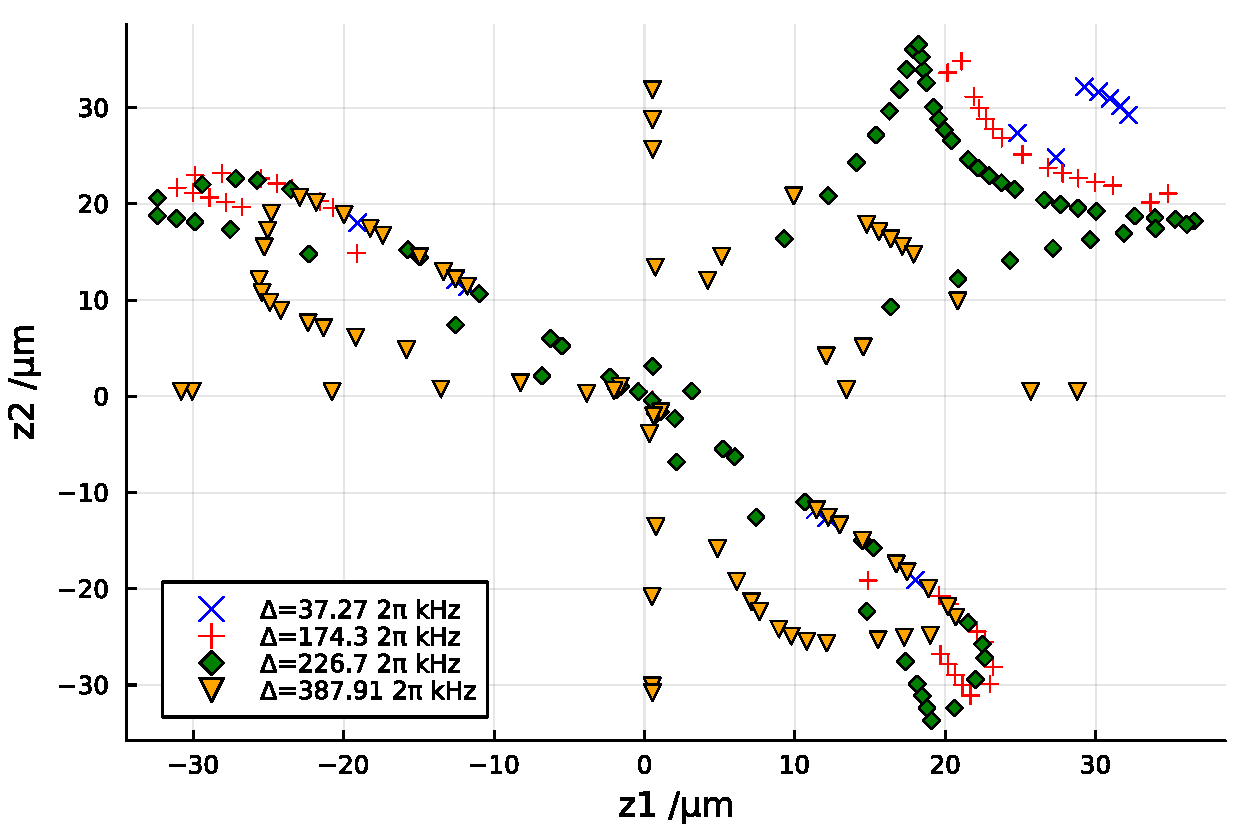
\includegraphics[width=0.8\linewidth]{chapters/12_2_particles/phi0.pdf}
        \caption{
            Plot the solutions of $\phi = 0$.
        }
        \label{fig:2p:phi0}
    \end{subfigure}
    \begin{subfigure}{\textwidth}
        \centering
        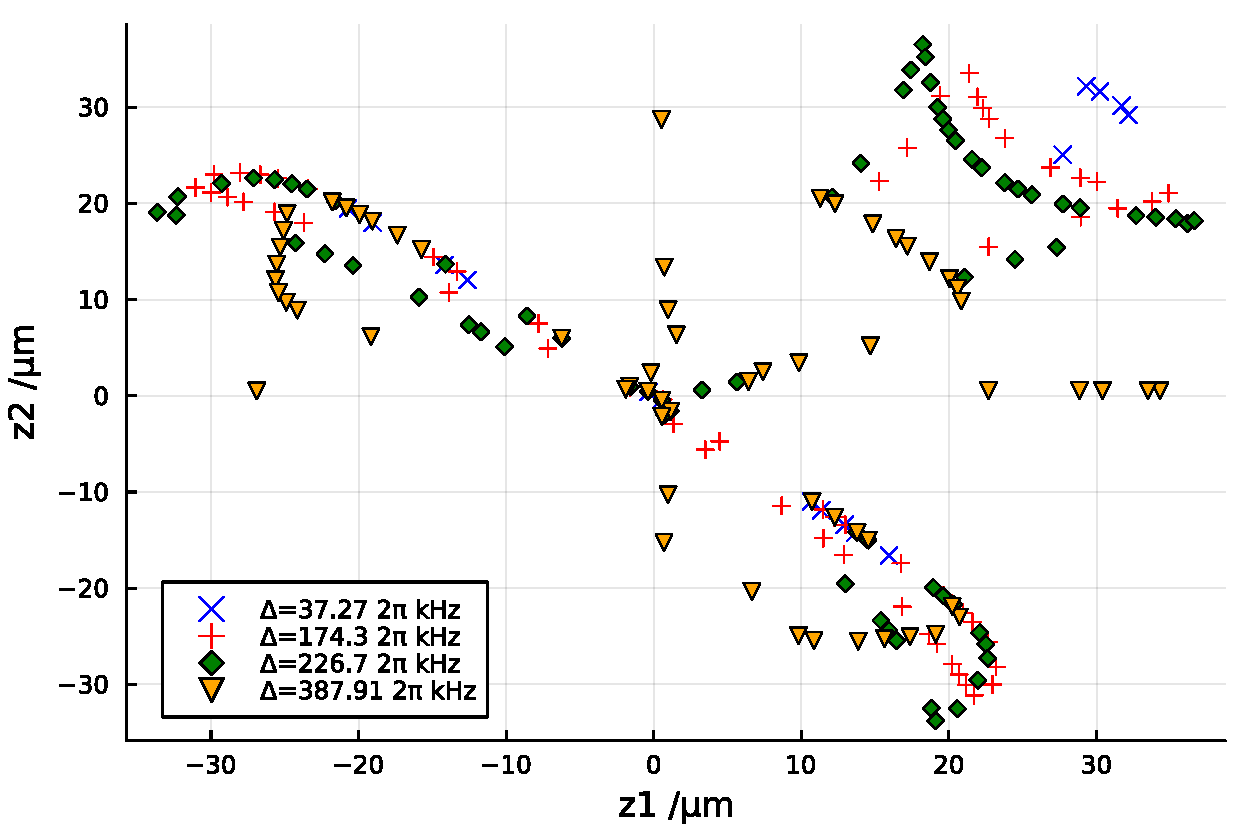
\includegraphics[width=0.8\linewidth]{chapters/12_2_particles/phi10.pdf}
        \caption{
            Plot the solutions of $\phi = \pi/10$
        }
        \label{fig:2p:phi10}
    \end{subfigure}
    \caption{
        Plots of different $\phi$ values at different detuning values.\\
        Additionally, $\kappa = 180~2\pi\unit{kHz}$ and the Parameters are from Table \ref{tab:sp:sim:params}.
    }
\end{figure}

\begin{figure}
     \centering
     \begin{subfigure}[b]{0.6\textwidth}
         \centering
         \includesvg[width=\textwidth]{chapters/12_2_particles/PlusPlusSector.svg}
         \caption{
            Symmetric case: $z_1 \sim z_2$
         }
         \label{fig:2p:hm:sym}
     \end{subfigure}
     \begin{subfigure}[b]{0.6\textwidth}
         \centering
         \includesvg[width=\textwidth]{chapters/12_2_particles/PlusMinusSector.svg}
         \caption{
            Antisymmetric Case: $z_1 \sim -z_2$
        }
         \label{fig:2p:hm:asym}
     \end{subfigure}
    \begin{subfigure}[b]{0.6\textwidth}
         \centering
         \includesvg[width=\textwidth]{chapters/12_2_particles/OnAxes.svg}
         \caption{
            Axes Case: $z_1 \sim 0$
        }
         \label{fig:2p:hm:axis}
     \end{subfigure}
     \caption{Heatmaps of $\norm{\vec L}^2$ }
            at $\Delta \simeq 387.91~2\pi\unit{kHz}$
     \label{fig:2p:hm}
\end{figure}
%We did the plots of the Solutions using Mathematica \cite{Mathematica} 
%    and its built in \lstinline{ContourPlot} \cite{reference.wolfram_2025_contourplot} function.
%For those plots we used the same parameters in Table \ref{tab:sp:sim:params}.
%Additionally we kept $\kappa = 180 ~2\pi \unit{kHz}$ and $\Delta = 100 ~2\pi \unit{kHz}$.
%We then plotted the results as $z_1$ vs $z_2$ using the \lstinline{ContourPlot} function.


